\section{Exploratory Data Analysis}
\vspace{-0.1in}

Exploratory data analysis (EDA) is an approach to analyze data sets and summarize their main characteristics. EDA is used for extracting information and visualization of it without involving the formal modeling or hypothesis testing task. It is an approach for data analysis that employs a variety of techniques to
\begin{itemize}
\item Maximize insight into a data set
\item Detect outliers and anomalies
\item Uncover underlying structure
\item Extract important variables
\item Test underlying assumptions
\item Develop economical models
\item Determine optimal factor settings
\end{itemize}

Most EDA techniques involve graphical representations with a few quantitative models. The reason for the heavy reliance on graphics is to open-mindedly explore data sets and it gives the analysts exceptional power to do so. It is enticing to reveal its structural secrets, and being always ready to gain some new, often unsuspected, insight into the data.
The particular graphical techniques employed in EDA are often quite simple, consisting of various techniques of:

\begin{itemize}
\item Plotting the raw data with techniques such as data traces, histograms, bihistograms, probability plots, log plots, block plots.
\item Plotting simple statistics such as mean plots, standard deviation plots, box plots, and main effects plots of the raw data.
\item Positioning such plots so as to maximize our natural pattern-recognition abilities, such as using different colors and types of plots for one type of data.
\end{itemize}


\subsection{Dataset Characteristics}
The training dataset provided by Kaggle contained 12 attributes (columns) with 891 records. These attributes included \textit{PassengerId,Survived,Pclass,Name,Sex,Age,SibSp,Parch,Ticket,Fare,Cabin and Embarked}. Here is a short description about each of the attributes/variables:
\begin{itemize}
\item Survived: Passenger survival. Takes value 0 for No and 1 for Yes.
\item Pclass: Passenger Class. Takes value 1 for 1st, 2 for 2nd and 3 for 3rd
\item name: Passenger Name
\item sex: Passenger Gender. Takes value male and female.
\item age: Passenger Age. Continuous variable takes non negative values.
\item sibsp: Number of Siblings/Spouses Aboard. Takes positive integral values.
\item parch: Number of Parents/Children Aboard. Takes positive integral values.
\item ticket: Passenger Ticket number.
\item fare: Passenger ticket fare. Continuous variable takes non negative values.
\item cabin: Passenger Cabin.
\item embarked: Port of Embarkation. Takes value C = Cherbourg, Q = Queenstown and S = Southampton.
\end{itemize}

Here are some of the special notes provided by Kaggle:
\begin{enumerate}
\item Pclass is a proxy for socio-economic status (SES). 1st ~ Upper; 2nd ~ Middle; 3rd ~ Lower

\item Age is in Years; Fractional if Age less than One (1). If the Age is Estimated, it is in the form xx.5

\item With respect to the family relation variables (i.e. sibsp and parch) some relations were ignored.  The following are the definitions used for sibsp and parch.
\begin{enumerate}

\item[Sibling:]  Brother, Sister, Stepbrother, or Stepsister of Passenger Aboard Titanic
\item[Spouse:]   Husband or Wife of Passenger Aboard Titanic (Mistresses and Fiances Ignored)
\item[Parent:]   Mother or Father of Passenger Aboard Titanic
\item[Child:]    Son, Daughter, Stepson, or Stepdaughter of Passenger Aboard Titanic

\end{enumerate}
\item Other family relatives excluded from this study include cousins,nephews/nieces, aunts/uncles, and in-laws.  Some children travelled only with a nanny, therefore parch=0 for them.  As well, some travelled with very close friends or neighbors in a village, however, the definitions do not support such relations.

\end{enumerate}

\subsection{Missing Data Completion}
While doing initial analysis, we observed that, for some variables, a lot values are not reported or are missing. The variables include Age, Cabin, Fare and Embarked. The variable Age is one of the most crucial variables amongst those specified as it plays significant role in prediction task (as will be observed later). These type of missing data are Missing at Random and can be estimated using different techniques as discussed below:
\begin{itemize}
\item Dropping Variables: We begin with dropping the data records with missing values and try getting insights into the data by plotting graph. However, since the a significant number of records have missing age values (almost 20\%), this method further worsens the training set. But it works fine with Cabin as almost 50\% of records having missing cabin values which restricts application of any other data completion technique. Embarked and Fare have only 1-2 records missing which don't really affect classification accuracy to a significant extent.
\item Mean: For age values, we take the mean value of non-missing values of age variable and assign it to all the missing records. As expected, this performs better and improves the correlation between this and variable to be predicted. We can similarly do the same for Embarked and Fare also. However, the thing to be noted here is that Embarked is categorical variable and so we assign the missing record the value which occurs most often. Furthermore, as we will see in the following sections, fare variable is not normally distributed and assigning mean to the missing record can prove to be misleading.
\item Class-wise mean: For age values, we observed through initial analysis that males have higher average/mean age values compared to females. Therefore, we calculated 2 different mean values one each for male and female by using the same method as mentioned in last point. We then assign the male average ages to the missing records with sex value as male and same for the females. It may not have created a significant impact on the classification accuracy, but it is considered as a good practice and can impact the accuracy if the data set is large.
\item Linear Regression: We then used a more complex way to estimate the missing age values. We applied linear regression to get the age values. However, this method had one serious drawback. Some of the values estimated were negative which poses serious problems to classifier. We used Scikit-Learn library in Python to implement regression.
\item ANOVA: As suggested in the Tutorials for Random Forest, we followed this method of regression for estimating the missing age values and it did perform well on that part.
\end{itemize}
\subsection{Feature Extraction}
There are various features that are considered for the analysis of data set such as the passenger class, age, gender etc. We consider each of them separately as follows:

\begin{figure}
\centering
\begin{minipage}{.5\textwidth}
  \centering
  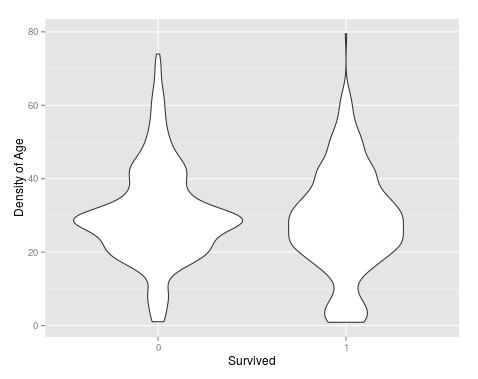
\includegraphics[width=1\linewidth]{figs/plot11}
  \captionof{figure}{Distribution of Age\\ in Survivors/Deaths}
  \label{fig:plot11}
\end{minipage}%
\begin{minipage}{.5\textwidth}
  \centering
  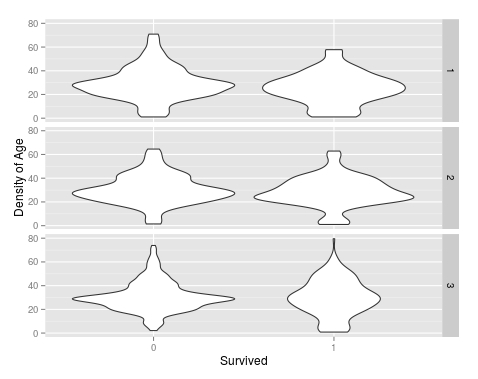
\includegraphics[width=1\linewidth]{figs/plot13}
  \captionof{figure}{Density of Age for Survivors/Deaths\\ in various classes (Voilin Plot)}
  \label{fig:plot13}
\end{minipage}
\end{figure}

\begin{figure}
\centering
\begin{minipage}{.5\textwidth}
  \centering
  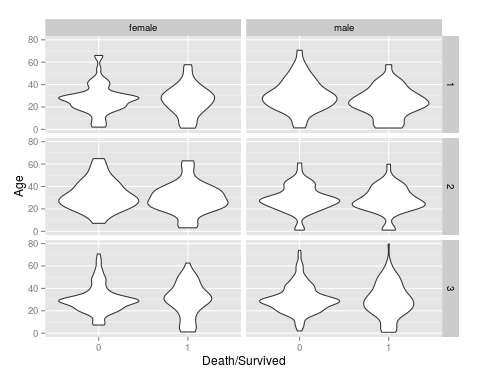
\includegraphics[width=1\linewidth]{figs/plot10}
  \captionof{figure}{Distribution of Age\\ for different Class and Gender}
  \label{fig:plot10}
\end{minipage}%
\begin{minipage}{.5\textwidth}
  \centering
  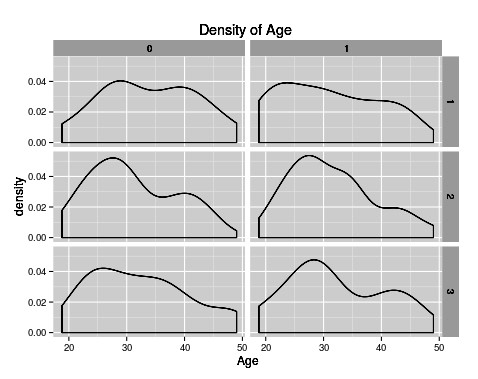
\includegraphics[width=1\linewidth]{figs/plot9}
  \captionof{figure}{Distribution of Middle Age(>20 \\and <50) Survivors/Deaths for different Class}
  \label{fig:plot9}
\end{minipage}
\end{figure}

\begin{figure}
\centering
\begin{minipage}{.5\textwidth}
  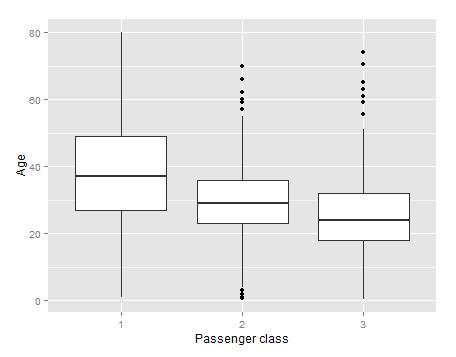
\includegraphics[width=1\linewidth]{figs/plot14}
  \captionof{figure}{Box plot for Passenger class vs Age}
  \label{fig:plot14}
\end{minipage}%
\begin{minipage}{.5\textwidth}
  \centering
  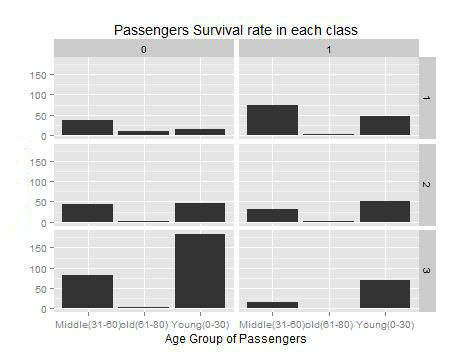
\includegraphics[width=1\linewidth]{figs/plot15}
  \captionof{figure}{Passenger Survivor for different\\ Age Groups and Class}
  \label{fig:plot15}
\end{minipage}
\end{figure}

We did some initial analysis of data as shown in the above Figures. Fig. \ref{fig:plot9},\ref{fig:plot10} \ref{fig:plot13} and \ref{fig:plot11} gave insights into the distribution of age seen from different angles. From these plots, we deduced that significant number of children(age<18) survived in Pclass 2 and 3. This helped in deciding one of the feature which is discussed in Random Forest model. Also, 1st and 2nd class senior citizens (age>50) were given preference as there are more survivors.

\begin{figure}
\centering
\begin{minipage}{.5\textwidth}
  \centering
  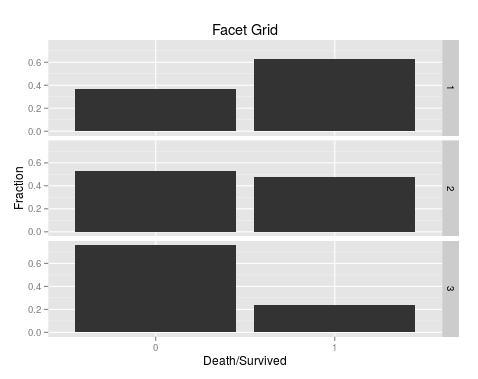
\includegraphics[width=1\linewidth]{figs/plot12}
  \captionof{figure}{Survivors/Deaths for different Pclass}
  \label{fig:plot12}
\end{minipage}%
\begin{minipage}{.5\textwidth}
  \centering
  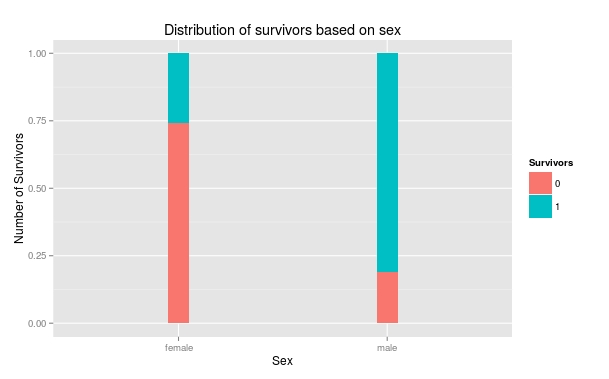
\includegraphics[width=1\linewidth]{figs/plot17}
  \captionof{figure}{Distribution of Survivors based\\ on Sex}
  \label{fig:plot17}
\end{minipage}
\end{figure}

\begin{figure}
\centering
\begin{minipage}{.5\textwidth}
  \centering
  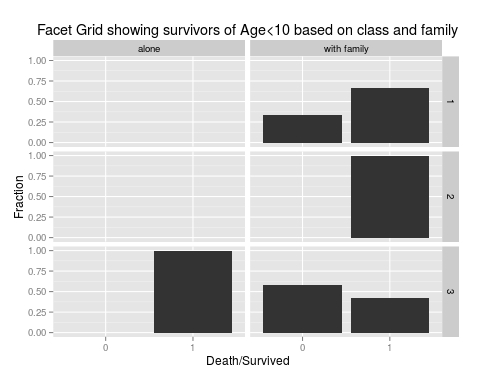
\includegraphics[width=1\linewidth]{figs/plot1}
  \captionof{figure}{Child(age<10) Survivors as\\ function of family and class}
  \label{fig:plot1}
\end{minipage}%
\begin{minipage}{.5\textwidth}
  \centering
  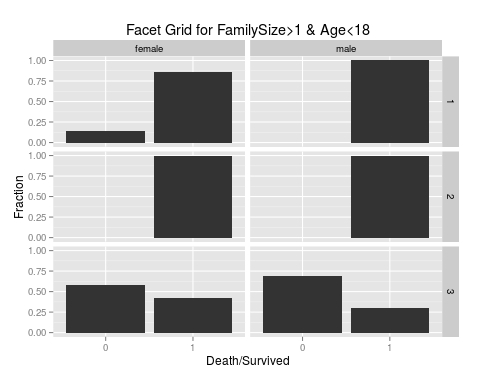
\includegraphics[width=1\linewidth]{figs/plot6}
  \captionof{figure}{Survivors as function of Family\\ and Age}
  \label{fig:plot6}
\end{minipage}
\end{figure}

Fig. \ref{fig:plot1} gave more insights into the child survivors when we saw its relationship with the family and class. As expected there were only a few children who were travelling alone. Almost all them were with family and their chances of survival also improved because of that. As can be seen, almost all of the 1st and 2nd class children survived the titanic crash.
Fig. \ref{fig:plot6} is one of the most crucial plot which helped us in improving the accuracy in Random Forest. This plot conveys that almost all the children(age<18) in 1st and 2nd class with familysize>1 survived the titanic crash.

\begin{figure}
\centering
\begin{minipage}{.5\textwidth}
  \centering
  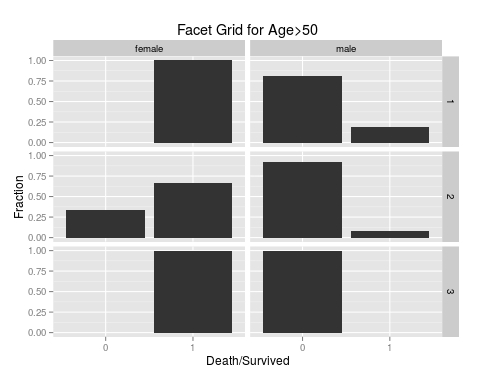
\includegraphics[width=1\linewidth]{figs/plot4}
  \captionof{figure}{Distribution of Survivors for\\ various class and Gender for\\ senior citizens (age>50)}
  \label{fig:plot4}
\end{minipage}%
\begin{minipage}{.5\textwidth}
  \centering
  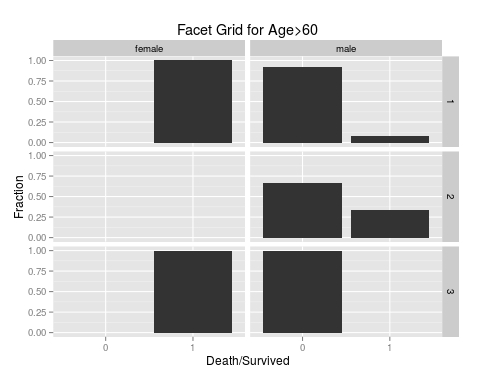
\includegraphics[width=1\linewidth]{figs/plot2}
  \captionof{figure}{Distribution of Survivors for\\ various class and Gender for\\ senior citizens (age>60)}
  \label{fig:plot2}
\end{minipage}
\end{figure}

Fig. \ref{fig:plot2} and \ref{fig:plot4} is in continuation with analysis done in various plots above. As can be seen from plot, almost all the females survived who have age>60 which was also one of our hypothesis as we know senior citizens were given preference. However, it is surprising to see that most of senior citizen males died. We extended the senior citizen age bar from 60 to 50 and it didn't have any significant difference.